\section{Solution}\label{solution}

%2.5 pages
%Renan: Solucao-Intro
%Renan: Solucao-Manipulator
%Estevão: Solucao-Rails (Renan revision)
%Estevão/Renan: Solucao-Shutter
%TODO Gabriel: Solucao-Calibration

The conceptual solution of EMMA is a mid-sized robotic manipulator with a
modular rail base. As the manipulator cannot fully cover the blade's surface in
a fixed position, and the robot locomotion is complex in the turbine's
environment, a customized rail is designed to provide extra degrees of
freedom (DOF) to the system. EMMA aims to be a generic solution to large bulb
type turbines, being modular, and versatile. The following system's elements
will be presented: the robotic manipulator; the customized base; and the robot
calibration.


\subsection{Robotic Manipulator}\label{manipulator}
The HVOF coating requirements and environment constraints demand a mid-sized
robotic manipulator (Sec.~\ref{hvof}), as a large-sized one would not
be able to move inside the confined space, and a small-sized manipulator would not
have the required payload and speed. In EMMA's project, the
robotic manipulator will be responsible for the coating application, precision, and tool handling.

A market survey is conducted to determine the most suitable robotic
manipulator for the application. Overall simu\-lations and analysis were performed using the OpenRave \cite{diankov2008openrave},
an environment for simulating motion planning algorithms for robotics. There are
several tools for dynamics simulation of robots: Gazebo, V-Rep,
Webots, MatLab/Simulink, and others% \cite{ivaldi2014tools}
. OpenRave stands out for having the following features: integral design for
real-time control and execution monitoring; core functionality for kinematics operations and
physics simulations; a network protocol allowing interpreted scripting languages
like Octave and Matlab; built-in core tools and plugin interfaces for
manipulation planning; standard plugins that allow testing of different planning
algorithms and sensing systems.

The simulations involve runner's blade discretization, base
position computations for full blade cover, and robotic manipulator's kinematics
and dynamics. 

The blade's surface discretization is an uniform sampling to
determine where to the coating directions should be. The current approach is to
take the bounding box of the blade and sample its surface uniformly. Once the
surface of the box is sampled, the intersection of the blade and a ray
originating from each point going inward is taken. The normal of the blade's
surface from each of these intersection points is taken to be the coating
direction. As an uniform sampling of the box does not mean an uniform sampling
of the blade, the box is oversampled and a 50~mm filter is applied, by a multidimensional search key with k-d tree.
The samples are translated 230~mm in respect with their normal vectors,
and collision checks with the environment are made. 

Base position computations are to uniformly sample the turbine's
confined space and to calculate the required robotic manipulator's base
positions to process all the samples (blade discretization),  considering angle
and distance tolerances. It is a brute force search: for each position, inverse
kinematics are computed to determine the robotic manipulator's joint parameters that provide
the desired positions and orientations of the end-effector.

The kinematic approach described above is not enough to ensure that the robot
will reach the samples. Maximum accelerations, decelerations,
torques, and jacobian singularities should be investigated and compared to the robotic
manipulator's specifications. The Newton-Euler method
\cite{sciavicco2000differential} was adopted for torque computation: $\tau =
M(q)\alpha + C(q,\omega)\omega + G(q)$, where $\tau$ is the joints' torques,
$M$ is the matrix of links' masses and moments of inertia, $\alpha$ is the
joints' accelerations, $q$ is the joints' angles, $\omega$ is the joints'
velocities, $C$ is the Coriolis matrix, and $G$ is the gravity vector.

In the dynamic approach, $M$ was estimated by the robotic manipulator's CAD
model. The angular accelerations are derived by differential kinematics:
$\alpha=J^+(a-\omega^TH\omega)$, where $H$ is the Hessian matrix
\cite{hourtash2005kinematic}, $a=\ddot{X}$ is the linear accelerations, and $J$
is the Jacobian matrix. Therefore, torques can be analytically estimated with
the inverse dynamics in OpenRave. 

% The typical path of HVOF coating is a zigzagging trajectory,
% i.e., it is a deceleration and acceleration process with direction changes. As
% the \textit{ex situ} solution uses a large-sized robotic manipulator, the
% end-effector's direction changes occur outside the blade's range, complying the
% speed requirement in the blade's range. However, while deceleration or
% acceleration, coating material is wasted to the environment or, most commonly,
% to a shadow plate.
% 
% The mid-sized robot for \textit{in situ} operation makes this strategy
% impossible, as, at some base positions, the robot will always be in the blade's
% range. The proposed solution modifies the original circuit of the gases that
% carry the coating particles to a new 2-way controlled circuit, in which there is
% a directional valve that changes the flow path from the thermal spray gun to return to tank
% circuit. The directional valve is autonomously actuated accordingly to the robotic
% manipulator's trajectory, i.e., the valve will ``shut'' while end-effector
% changes its direction. Therefore, the solution provides coating material
% savings, as the non-used particles are stored for future usage, and the hard
% coating speed requirement is met.

% \begin{figure}[h!]
%    \centering
%    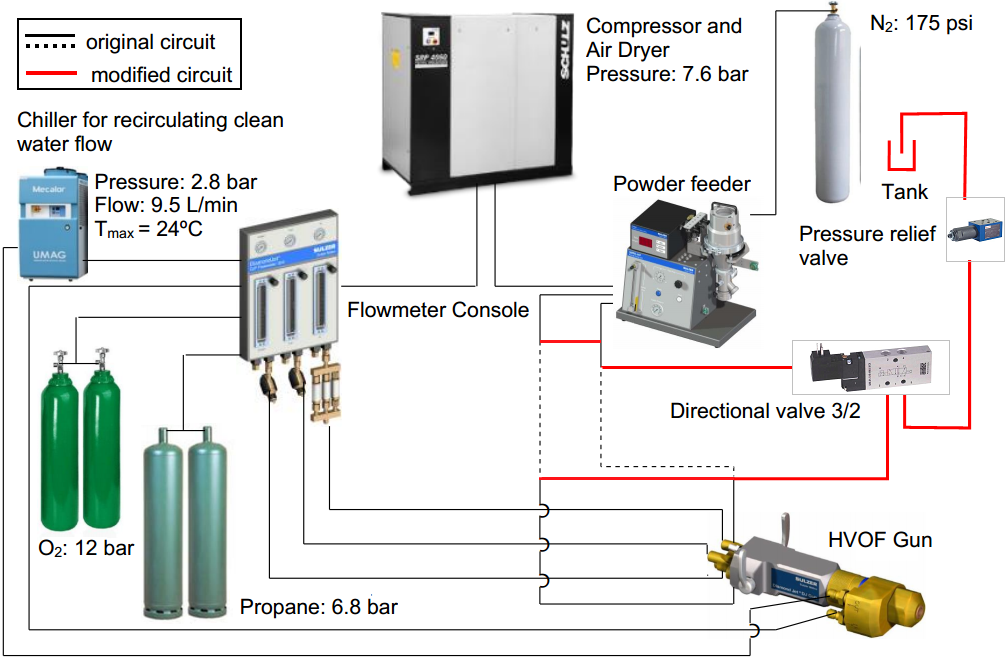
\includegraphics[width=0.9\columnwidth]{figs/mecanica/Circuito_HVOF_mod_en.PNG}
%    \caption{Simplified view of HVOF circuit with shutter}
%    \label{fig::circuito_hvof}
% \end{figure}

 

\subsection{Base}
% 0.75 pages

EMMA's base comprises two rails, forming two prismatic joints (P). The
first, or primary rail, is parallel to the turbine axis, and it is responsible
for the transportation of the robotic manipulator from hatch to blade. The
secondary rail is parallel to the blade's surface, and it is assembled from the
first rail by a rotational joint (R).

\begin{figure}
	\centering
	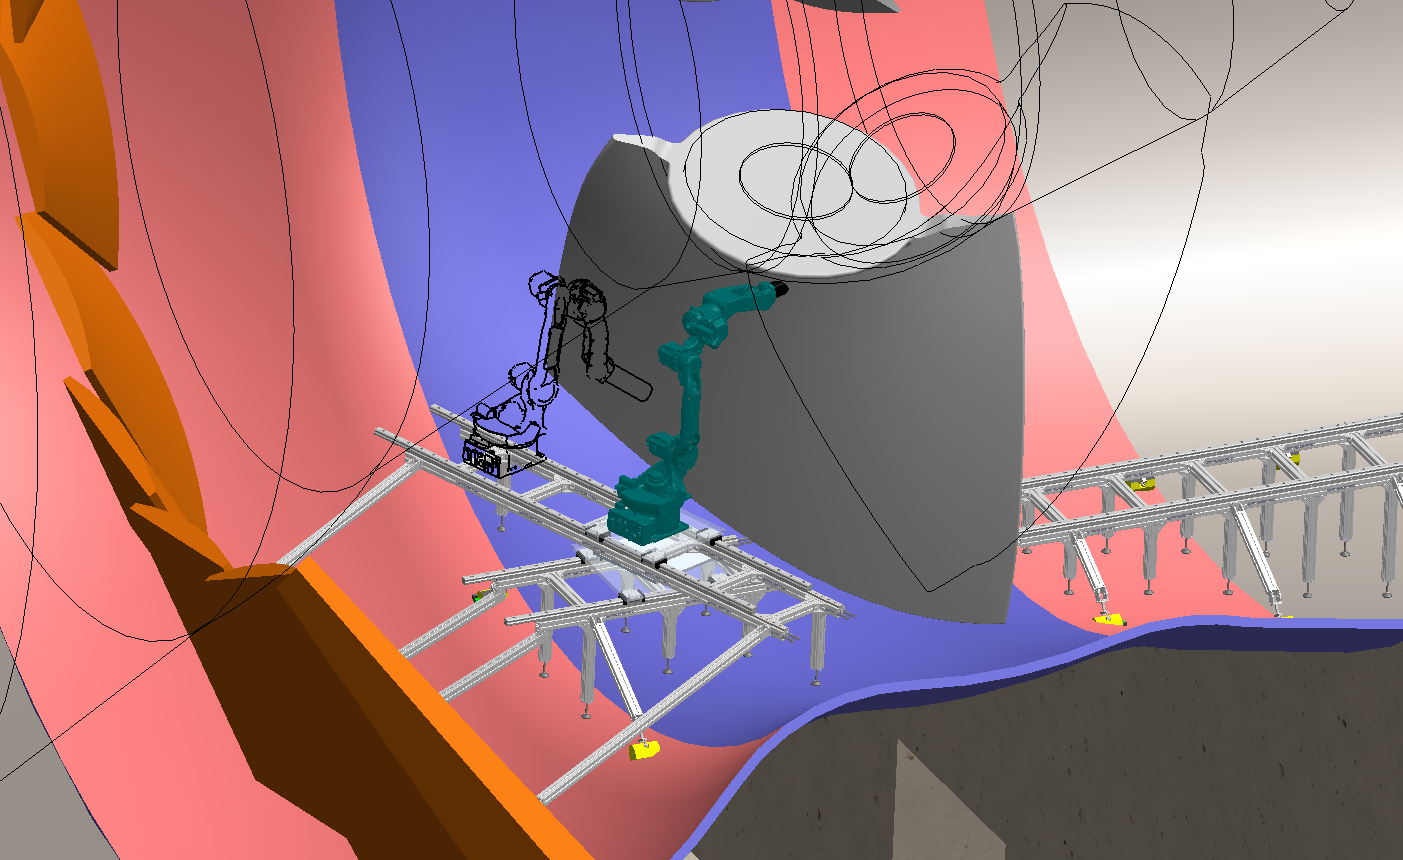
\includegraphics[width=.8\columnwidth]{figs/mecanica/EMMA_Base_Secundaria_01.PNG}
    \caption{Customized base: primary and secondary rails.}
    \label{fig:base}
\end{figure}

The hatch and turbine' space can limit the size of the rail in terms of weight
and geometry, thus a modular concept was design, such that the small modular parts can be easily and
manually assembled inside the turbine. The base is a modular two parallel
profiled rail with a four carriage setup%  \cite{SKF_2013}
. In this
configuration, the reaction moments of the base are cancelled by a force couple provided by each couple of
carriages. The commercial modules are aluminum structures for corrosion resistance,
lightweight, geometric flexibility, and modularity, as it is possible to
increase/decrease the rail length/width/height by changing few parts or adding
anchor arms.

The resulting base is a slender and lightweight frame, such that a careful
analysis is necessary to evaluate the structural integrity and rigidity in
respect to the dynamic loads of the robotic manipulator. A Finite Element
Analysis (FEA) was performed to study the stresses, strains and resultant forces
along the structure. FEA is also used to size the frame components, such as
the profile's size, and to size the anchors, its directions, and attachment to
provide the greater base's rigidity. The rigidity is a major concern, it is
required for the hard coating process, since a non-rigid base propagates
vibrations to the robotic manipulator's end-effector with high amplitudes, which
may compromise coating quality.

The draft tube and runner area are conical shape structures, curved and
sloped. The environment modification, as wielding and drilling, should be
avoided, thus properly fixing the base on the ground is a major challenge in
EMMA project. The draft tube is composed of a ferromagnetic steel material,
hence magnetic fixtures is suitable for base attachment. 

\begin{comment}
Common magnetic fixture products are temporary magnetic equipments used to hoist
and transport materials in an industrial plant. In EMMA, it is used to attach
and anchor the rail's modules to the ground.
\end{comment}

\subsection{Calibration}

In opposition to \textit{ex situ} operations, in which the relative position
between the robot and the blade to be coated is fixed and \textit{a prior}
known, \textit{in situ} operations this assumptions cannot be made and it
is needed to aquire information from the environment in order to identify
and localize the elements of interest. In EMMA, the system calibration consists
in the indentification of the manipulator and blade, and their
pose estimation in respect to the turbine interior. Due the light conditions
inside the hydraulic circuit  a 3D laser scanner is used to gather
tridimensional information of the environment, including the robot manipulator
and base. The calibration process was divided in two different approach
depending on the element to be localized and its caracteristics. The possibility
to attach or install markers in known positions dictated the strategies to be
chosen, therefore the calibration is separeted in the pose estimation of the
robot and of the blade, as follows.
 
The attachment of markers on the robotic manipulator can be performed with high
precision and repeatability, thus reflective spheres were chosen as reference
points in the process of robot localization. These spheres are identified inside
the point cloud by a 3D Hough transform method \cite{camurri20143d}.

Alternatively, to install any marker on the
blade would require its own calibration to ensure a consistent reference point,
therefore the pose estimation of the blade must rely only on the intrinsec
properties of the its surface geometry. The information must be extracted from
the point cloud provided by the 3d laser sensor and compared to a reference
model previously stored. The characteristics of the point clouds are represented
by local descriptors, i.e., each point of interest on the blade is associated
with the information about its local neighborhood. Given the
sets of features,  it is possible to determine the correspondence between the
two sets. If enough correspondences are found in the scene, above a threshold,
the blade is identified and the position is determined \cite{Tombari2010a}. 

The computation of the descriptors is expensive and a subsampling of the point
clouds, both model and the scene, is perfomed due the high density provided by
the sensor. However, considering the geometry of the reference model searched
in the scene, i.e. the blade, it is fundamental to pick wisely the interest
points that will have a descriptor associated, as the blade is has a large area
with a smooth surface and the neighborhood of each point on this section
introduce similiar information, creating ambiguous descriptors that degrade the
matching perfomance between the two point clouds.
The samples in this area can only provide information about the translation in
the direction perpendicular to the supporting plane and the two rotation
associated with it, there is no information about the others DoF, making the
alingment to ``slide'' from the correct transformation. Therefore, the interest
points were sampled in order to keep the distribution of normals as large as
possible \cite{Rusinkiewicz2001}. This approach enables the reduction of the
number of points to be sampled and has a lower computional cost.

Once the the descriptors were estimated the correspondences between them are
determined if the euclidean distance between a descriptor in the scene and model
is lower than a threshold. Each Correspondence vote, then, for a specific pose
and scale factor in the Hough space. After the an instance of the model is
found, it is performed an ICP matching with the full resolution point clouds to
realize a fine alignment and compensate any discrepancy introduced by the
sampling. With the position of the blade and the manipulator in respect to a
common coordinate system, i.e. the origin of the laser sensor, it is possible to
determine the transformation between them and this information can be fed to the
trajectory and coverage algorithms.



